%!TEX TS-program = xelatex
\documentclass[12pt, a4paper, oneside]{article}

% пакеты для математики
\usepackage{amsmath,amsfonts,amssymb,amsthm,mathtools}  
\mathtoolsset{showonlyrefs=true}  % Показывать номера только у тех формул, на которые есть \eqref{} в тексте.

\usepackage[english, russian]{babel} % выбор языка для документа
% \usepackage[utf8]{inputenc}          % utf8 кодировка

% Основные шрифты 
\usepackage{fontspec}         
\setmainfont{Linux Libertine O}  % задаёт основной шрифт документа

% Математические шрифты 
\usepackage{unicode-math}     
\setmathfont[math-style=upright]{[Neo Euler.otf]} 


%%%%%%%%%% Работа с картинками и таблицами %%%%%%%%%%
\usepackage{graphicx} % Для вставки рисунков                
\usepackage{graphics}
\graphicspath{{images/}{pictures/}}   % папки с картинками

\usepackage{wrapfig}    % обтекание рисунков и таблиц текстом

\usepackage{booktabs}   % таблицы как в годных книгах
\usepackage{tabularx}   % новые типы колонок
\usepackage{tabulary}   % и ещё новые типы колонок
\usepackage{float}      % возможность позиционировать объекты в нужном месте
\renewcommand{\arraystretch}{1.2}  % больше расстояние между строками


%%%%%%%%%% Графики и рисование %%%%%%%%%%
\usepackage{tikz, pgfplots}  % языки для графики
\pgfplotsset{compat=1.16}

\usepackage{todonotes} % для вставки в документ заметок о том, что осталось сделать
% \todo{Здесь надо коэффициенты исправить}
% \missingfigure{Здесь будет Последний день Помпеи}
% \listoftodos --- печатает все поставленные \todo'шки


%%%%%%%%%% Внешний вид страницы %%%%%%%%%%

\usepackage[paper=a4paper, top=20mm, bottom=15mm,left=20mm,right=15mm]{geometry}
\usepackage{indentfirst}    % установка отступа в первом абзаце главы

\usepackage{setspace}
\setstretch{1.15}  % межстрочный интервал
\setlength{\parskip}{4mm}   % Расстояние между абзацами
% Разные длины в LaTeX: https://en.wikibooks.org/wiki/LaTeX/Lengths

% свешиваем пунктуацию
% теперь знаки пунктуации могут вылезать за правую границу текста, при этом текст выглядит ровнее
\usepackage{microtype}

% \flushbottom                            % Эта команда заставляет LaTeX чуть растягивать строки, чтобы получить идеально прямоугольную страницу
\righthyphenmin=2                       % Разрешение переноса двух и более символов
\widowpenalty=300                     % Небольшое наказание за вдовствующую строку (одна строка абзаца на этой странице, остальное --- на следующей)
\clubpenalty=3000                     % Приличное наказание за сиротствующую строку (омерзительно висящая одинокая строка в начале страницы)
\tolerance=10000     % Ещё какое-то наказание.

% мои цвета https://www.artlebedev.ru/colors/
\definecolor{titleblue}{rgb}{0.2,0.4,0.6} 
\definecolor{blue}{rgb}{0.2,0.4,0.6} 
\definecolor{red}{rgb}{1,0,0.2} 
\definecolor{green}{rgb}{0,0.6,0} 
\definecolor{purp}{rgb}{0.4,0,0.8} 

% цвета из geogebra 
\definecolor{litebrown}{rgb}{0.6,0.2,0}
\definecolor{darkbrown}{rgb}{0.75,0.75,0.75}

% Гиперссылки
\usepackage{xcolor}   % разные цвета

\usepackage{hyperref}
\hypersetup{
	unicode=true,           % позволяет использовать юникодные символы
	colorlinks=true,       	% true - цветные ссылки
	urlcolor=blue,          % цвет ссылки на url
	linkcolor=red,          % внутренние ссылки
	citecolor=green,        % на библиографию
	breaklinks              % если ссылка не умещается в одну строку, разбивать её на две части?
}

% меняю оформление секций 
\usepackage{titlesec}
\usepackage{sectsty}

% меняю цвет на синий
\sectionfont{\color{titleblue}}
\subsectionfont{\color{titleblue}}

% выбрасываю нумерацию страниц и колонтитулы 
\pagestyle{empty}

% синие круглые бульпоинты в списках itemize 
\usepackage{enumitem}

\definecolor{itemizeblue}{rgb}{0, 0.45, 0.70}

\newcommand*{\MyPoint}{\tikz \draw [baseline, fill=itemizeblue, draw=blue] circle (2.5pt);}

\renewcommand{\labelitemi}{\MyPoint}

% расстояние в списках
\setlist[itemize]{parsep=0.4em,itemsep=0em,topsep=0ex}
\setlist[enumerate]{parsep=0.4em,itemsep=0em,topsep=0ex}


%%%%%%%%%% Свои команды %%%%%%%%%%

% Математические операторы первой необходимости:
\DeclareMathOperator{\sgn}{sign}
\DeclareMathOperator*{\argmin}{arg\,min}
\DeclareMathOperator*{\argmax}{arg\,max}
\DeclareMathOperator{\Cov}{Cov}
\DeclareMathOperator{\Var}{Var}
\DeclareMathOperator{\Corr}{Corr}
\DeclareMathOperator{\E}{\mathop{E}}
\DeclareMathOperator{\Med}{Med}
\DeclareMathOperator{\Mod}{Mod}
\DeclareMathOperator*{\plim}{plim}

% команды пореже
\newcommand{\const}{\mathrm{const}}  % const прямым начертанием
\newcommand{\iid}{\sim i.\,i.\,d.}  % ну вы поняли...
\newcommand{\fr}[2]{\ensuremath{^{#1}/_{#2}}}   % особая дробь
\newcommand{\ind}[1]{\mathbbm{1}_{\{#1\}}} % Индикатор события
\newcommand{\dx}[1]{\,\mathrm{d}#1} % для интеграла: маленький отступ и прямая d

% одеваем шапки на частые штуки
\def \hb{\hat{\beta}}
\def \hs{\hat{s}}
\def \hy{\hat{y}}
\def \hY{\hat{Y}}
\def \he{\hat{\varepsilon}}
\def \hVar{\widehat{\Var}}
\def \hCorr{\widehat{\Corr}}
\def \hCov{\widehat{\Cov}}

% Греческие буквы
\def \a{\alpha}
\def \b{\beta}
\def \t{\tau}
\def \dt{\delta}
\def \e{\varepsilon}
\def \ga{\gamma}
\def \kp{\varkappa}
\def \la{\lambda}
\def \sg{\sigma}
\def \tt{\theta}
\def \Dt{\Delta}
\def \La{\Lambda}
\def \Sg{\Sigma}
\def \Tt{\Theta}
\def \Om{\Omega}
\def \om{\omega}

% Готика
\def \mA{\mathcal{A}}
\def \mB{\mathcal{B}}
\def \mC{\mathcal{C}}
\def \mE{\mathcal{E}}
\def \mF{\mathcal{F}}
\def \mH{\mathcal{H}}
\def \mL{\mathcal{L}}
\def \mN{\mathcal{N}}
\def \mU{\mathcal{U}}
\def \mV{\mathcal{V}}
\def \mW{\mathcal{W}}

% Жирные буквы
\def \mbb{\mathbb}
\def \RR{\mbb R}
\def \NN{\mbb N}
\def \ZZ{\mbb Z}
\def \PP{\mbb{P}}
\def \QQ{\mbb Q}


%%%%%%%%%% Теоремы %%%%%%%%%%
\theoremstyle{plain} % Это стиль по умолчанию.  Есть другие стили.
\newtheorem{theorem}{Теорема}[section]
\newtheorem{result}{Следствие}[theorem]
% счётчик подчиняется теоремному, нумерация идёт по главам согласованно между собой

% убирает курсив и что-то еще наверное делает ;)
\theoremstyle{definition}         
\newtheorem*{definition}{Определение}  % нумерация не идёт вообще


%%%%%%%%%% Задачки и решения %%%%%%%%%%
\usepackage{etoolbox}    % логические операторы для своих макросов
\usepackage{environ}
\newtoggle{lecture}

\newcounter{problem}%[section]  % счётчик для упражнений 

\renewcommand{\theproblem}{\arabic{problem}}

\newenvironment{problem}{
\addtocounter{problem}{1}\noindent{ \color{titleblue} \large \bfseries Упражнение~\theproblem \vspace{1ex} \newline}
}{ }

% Окружение, чтобы можно было убирать решения из pdf
\NewEnviron{solution}{%
  \iftoggle{lecture}
    {\noindent \textbf{\large Решение:} \vspace{1ex} \newline \BODY}
    {}%
  }
  
% выделение по тексту важных вещей
\newcommand{\indef}[1]{\textbf{ \color{green} #1}} 

% эпиграфы
\usepackage{epigraph}
\setlength\epigraphwidth{.4\textwidth}
\setlength\epigraphrule{0pt}

\begin{document} % Конец преамбулы, начало файла

% Если переключить в false, все solution исчезнут из pdf
\toggletrue{lecture}
%\togglefalse{lecture}


\section*{Семинар 3: основы статистики!}

\epigraph{Безумная цитата}{автор этой цитаты}

% \todo[inline]{Так можно делать заметки для меня}

В первом разделе семинара большая задачка, которую мы с вами решали на паре. 

\begin{problem}
Коллекционер Настя собрала целых $10$ наблюдений и записала их в табличку. Теперь Настя хочет стать аналитиком и проанализировать таблицу. Помогите ей. 

\begin{center}
	\begin{tabular}{lccc}
		\toprule
		имя & пол  & возраст  & вес  \\ \midrule
		Кхал & м  & $14$ &   $80$  \\
		Санса & ж & $15$ &  $40$  \\
		Мелисандра & ж & $21$ &  $40$   \\
		Эддард & м & $20$ &   $80$ \\
		Сандор & м & $14$ &   $80$ \\
		Миссандея & ж & $25$ &   $40$\\
		Якен & м & $30$ &   $80$\\
		Теон & ж & $23$ &    $40$\\
		Тирион & м & $22$ &    $80$\\
		Станис & м & $16$  &    $440$\\ \bottomrule
	\end{tabular}	
\end{center}

\begin{enumerate}
	\item[а)] Что такое непрерывная переменная? Что такое категориальная переменная? Какие переменные в табличке относятся к непрерывным? Какие к категориальным?  Приведите ещё примеров непрерывных и категориальных переменных! 
	
	\item[б)]  Найдите долю мужчин и женщин в выборке. Постройте для пола гистограмму. 
	
	\item[в)] Найдите средний возраст и медианный возраст.  Что означают эти числа. В чём они измеряются? 

	\item[г)] Найдите дисперсию возраста. В чём измеряется эта величина? Зачем обычно ищут среднее квадратичное отклонение? Найдите его. 	
	
	\item[д)]  Постройте гистограмму для возраста. Считайте, что ширина одного столбца --- 5 лет. Если человек попадает на правую границу отрезка, он попадает в текущий столбец.  Изобразите на гистограмме среднее, медиану. Как бы вы нарисовали на гистограмме стандартное отклонение? 
	
	\item[е)] Что такое выброс? Есть ли выбросы в возрасте? Есть ли выбросы в весе? Как выглядит выброс на гистограмме? Найдите средний вес и медианный вес. Чем медиана в данном случае лучше, чем среднее?
	
	\item[ж)] Чувствительна ли дисперсия к выбросам?
	
	\item[з)] Что такое мода? Почему использовать её для непрерывных переменных не очень хорошая идея? Найдите моду для имени, пола и возраста.
	
	\item[и)]  Что такое квантиль? Предложите способ  борьбы с выбросами, основанный на знании того, что такое квантиль.
\end{enumerate}
\end{problem}

\begin{solution}
\begin{enumerate}
	\item[а)] \indef{Непрерывная переменная} не ограничена каким-то конечным набором значений и может принимать любые числовые значения. Например: цена на квартиру, валютный курс, возраст, число лайков под фоткой и т.п. 
	
	\indef{Категориальная переменная} принимает значения из какого-то фиксированного конечного множества. Например: пол, марка машины и тп.
	
	\item[б)]  В выборке $6$ мужчин и $4$ женщины.  Всего $10$ человек.  Значит доля мужчин $\frac{6}{10} = 0.6$, доля женщин $\frac{4}{10} = 0.4$. Нарисуем гистограмму. По оси $x$ будем откладывать возможные значения для нашей переменной, по оси $y$ насколько часто это значение наблюдается в выборке. 
	
	\begin{center}
	\begin{tikzpicture}[line cap=round,line join=round,x=1.0cm,y=1.0cm]
	\draw [color=darkbrown,xstep=1.0cm,ystep=1.0cm] (-3.,-0.04) grid (5.04,5.96);
	\clip(-3.,-0.04) rectangle (5.04,5.96);
	\fill[line width=2.pt,color=litebrown,fill=litebrown,fill opacity=0.10000000149011612] (-1.,1.) -- (-1.,4.) -- (0.,4.) -- (0.,1.) -- cycle;
	\fill[line width=2.pt,color=litebrown,fill=litebrown,fill opacity=0.10000000149011612] (1.,1.) -- (1.,3.) -- (2.,3.) -- (2.,1.) -- cycle;
	\draw [->,line width=2.pt] (-1.98,0.42) -- (-2.,5.);
	\draw [->,line width=2.pt] (-2.54,1.) -- (4.,1.);
	\draw [line width=2.pt,color=litebrown] (-1.,1.)-- (-1.,4.);
	\draw [line width=2.pt,color=litebrown] (-1.,4.)-- (0.,4.);
	\draw [line width=2.pt,color=litebrown] (0.,4.)-- (0.,1.);
	\draw [line width=2.pt,color=litebrown] (0.,1.)-- (-1.,1.);
	\draw [line width=2.pt,color=litebrown] (1.,1.)-- (1.,3.);
	\draw [line width=2.pt,color=litebrown] (1.,3.)-- (2.,3.);
	\draw [line width=2.pt,color=litebrown] (2.,3.)-- (2.,1.);
	\draw [line width=2.pt,color=litebrown] (2.,1.)-- (1.,1.);
	\draw (-2.5,5.5) node[anchor=north west] {$y$};
	\draw (4.1,1.32) node[anchor=north west] {$x$};
	\draw (-1.5,0.7) node[anchor=north west] {\text{мужчины}};
	\draw (0.6,0.7) node[anchor=north west] {\text{женщины}};
%	\draw [line width=2.pt,dash pattern=on 2pt off 2pt] (-1.,4.)-- (-2.,4.);
%	\draw [line width=2.pt,dash pattern=on 2pt off 2pt] (1.,3.)-- (-2.,3.);
	\draw (-2.5,4.5) node[anchor=north west] {$6$};
	\draw (-2.5,3.5) node[anchor=north west] {$4$};
	\draw (-2.5,2.5) node[anchor=north west] {$2$};
	\draw (-2.5,1.6) node[anchor=north west] {$0$};
	\end{tikzpicture}
	\end{center}
	
	\item[в)]  Найдём \indef{средний возраст.} Для этого сложим все числа и поделим их на количество наблюдений
	
	\[
	\frac{1}{10} \cdot (14 + 15 + 20 + 21 + 14 + 25 + 30 + 23 + 22 + 16) = 20.
	\]
	
	Средний возраст это $20$ лет.  Формула для подсчёта среднего выглядела так:
	
	\[
	\bar x = \frac{1}{n} (x_1 + \ldots + x_n) = \frac{1}{n} \sum_{i=1}^n x_i.
	\]
	
	Привыкайте к формулам. Они будут часто встречаться вам по жизни. 
	
	Чтобы найти медиану, нам нужно упорядочить всех людей из выборки по возрасту и посмотреть какое число оказалось в середине:
	
	\[
	14 \quad 14  \quad 15  \quad 16  \quad {\color{purp}{20}}  \quad {\color{purp}{21}}  \quad 22  \quad 23  \quad 25  \quad 30
	\]
	
	У нас в середине находятся сразу два числа. В случаях, когда такое происходит в качестве медианы берут среднее этих двух чисел. В нашем случае это $\fr{1}{2} \cdot (20 + 21) = 20.5$. Медиана это число, взятое посередине. Половина выборки оказывается слева от него, а вторая половина справа. Среднее и медиана в нашей задачке измеряются в годах и обозначают типичный возраст, который присущ людям из выборки. 
	
	\item[г)]  \indef{Дисперсия} --- это мера разброса. Она показывает насколько разнообразными могут быть элементы в выборке, насколько сильно они могут отклоняться от своего типичного значения. 
	
	Чтобы найти её, нужно посмотреть насколько сильно каждый представитель в выборке отличается от текущего. Величина такого отличия называется отклонением.
	
	Предположим, что Алёне и Карине обеим по $18$ лет. При рассмотрении этих двух человек средний возраст вычисляется как средняя сумма двух слагаемых: $\frac{18 + 18}{2} = 18$. Тогда отклонением для Алёны и Карины от среднего возраста будет $18 - 18 = 0$ года, а среднее отклонение нулевое: $\frac{0 + 0}{2}$. То есть в нашей выборке из двух человек нет неоднородности, у всех людей одинаковый возраст.
	
	Предположим теперь, что Алёне $18$ лет, а Карине $22$ года. Средний возраст всё ещё вычисляется как средняя сумма двух слагаемых: $\frac{18 + 22}{2} = 20$. Тогда отклонением для Алёны от среднего возраста будет $18 - 20 = -2$ года. Для Карины отклонением будет $22 - 20 = 2$ года. 
	Если посчитать среднее этих отклонений, мы получим $\frac{-2 + 2}{2} = 0$. То есть в выборке нет никакого разброса. Все люди не отличаются от среднего. Это неправда.
	
	Для того, чтобы избежать неправды и жить по правде, отклонения возводят в квадрат, тогда мы получаем, что суммарное отклонение будет $(-2)^2 + 2^2 = 4 + 4 = 8$. Посмотрев на такое число мы сразу же поймём, что в выборке есть неоднородность. 
	
	Среднее значение квадратов отклонений от среднего и называется дисперсией. Давайте найдём её. Ещё раз выпишем наши наблюдения: 
	
	\[
	14 \quad 14  \quad 15  \quad 16  \quad 20  \quad 21  \quad 22  \quad 23  \quad 25  \quad 30
	\]
	
	Сначала из каждого вычитаем среднее. Это даст нам
	
	\[
	-6 \quad -6  \quad -5  \quad -4  \quad 0  \quad 1 \quad 2  \quad 3  \quad 5  \quad 10.
	\]
	
	Теперь возводим все отклонения в квадрат
	
	\[
	36 \quad 36  \quad 25  \quad 16 \quad 0  \quad 1 \quad 4  \quad 9 \quad 25  \quad 100.
	\]
	
	Складываем их.  Получается $252$. Остаётся разделить это число на  $10$ (количество наблюдений). Получается, что дисперсия составит $25.2$ квадратных года.  Из-за того, что мы каждое слагаемое возводили в квадрат, \indef{дисперсия измеряется в квадратных годах.}
	
	Когда мы умножаем одну сторону квадрата, измеренную в метрах, на другую, мы получаем его площадь. Она измеряется в квадратных метрах. Тут похожая ситуация. Мы бы хотели вернуться назад, к обычным годам. Для этого из дисперсии извлекают корень и получают штуку под названием стандартное отклонение. В нашем случае получится $\sqrt{25.2} \approx 5.02$ года. 
	
	
	Можно найти дисперсию проще и быстрее. Для этого есть специальная формула: 

	$$
	\hat \sigma^2 = \overline{x^2} - (\bar x)^2,
	$$
	
	то есть дисперсия это среднее квадратов минус квадрат среднего. Эту формулу довольно просто доказать. На матстате вы её докажете. А пока просто воспользуемся ей. Найдём квадрат среднего:
	
	$$
	(\bar x)^2 = 20^2 = 400
	$$
	
	Теперь среднее квадратов: 
	
	$$
	\overline{x^2} = \frac{1}{10} \cdot (14^2 + 15^2 + 21^2 + 20^2 + 14^2 + 25^2 + 30^2 + 23^2 + 22^2 + 16^2) = 425.2.
	$$
	
	Остался последний штрих: 
	
	$$
	\hat \sigma^2 = 425.2 - 400 = 25.2.
	$$
	
	Пользуйтесь тем способом, который вам больше нравится. Про дисперсию давайте обсудим ещё пару дополнительных полезных нюансов: 
	
	\begin{itemize}
		\item  Мы возводим отклонения в квадрат не только для того, чтобы сделать все числа положительными. Попутно мы подчёркиваем, что чем больше отклоняется возраст от среднего, тем это хуже. Так штраф за отклонение в два года составит $4$, а за отклонение в три года штраф будет $9$.  С подобной логикой мы ещё встретимся, когда будем обсуждать различные метрики, используемые в машинном обучении. 
		
		\item Часто при подсчёте дисперсии вместо формулы 
		
		\[ 
		\hat \sigma^2 = \frac{1}{n} \sum_{i=1}^n (x_i - \bar x)^2,
		\]
		
		которую использовали мы, используют 
		
		\[ 
		\hat \sigma^2 = \frac{1}{n-1} \sum_{i=1}^n (x_i - \bar x)^2.
		\]
		
		\indef{Вторая формула, на самом деле, корректнее, чем первая.} В \textit{pandas} используется именно она. У этого есть глубокая причина, которая называется несмещённостью оценки. В полной мере вы узнаете про это в курсе по математической статистике. Мы вкратце поговорим про несмещённые оценки ближе к концу курса, когда будем говорить про АБ-тесты. Пока держите это в голове, как вопрос, на который у вас нет ответа. Надеюсь, что это будет как следует мучать вас по ночам и стимулировать ботать. 
	
		\item Если распределение у данных \textit{нормальное}*, тогда  большая часть выборки, а именно $69\%$ кучкуется в диапазоне между $\bar x - \hat \sigma$ и $\bar x + \hat \sigma$.  
		
		При этом $95 \%$ выборки находится между $\bar x - 2 \cdot \hat \sigma$ и $\bar x + 2 \cdot \hat \sigma$, а $99.9\%$ выборки находятся между $\bar x - 3 \cdot \hat \sigma$ и $\bar x + 3 \cdot \hat \sigma$. 
		
		Правила таких кучкований называют правилом одной, двух и трёх сигм. Их часто используют для проведения АБ-тестов. Об этом мы тоже поговорим ближе к концу курса.

		* Что такое \textit{нормальное распределение} --- отдельный и очень важный вопрос. Пока можно держать в голове, что, если выборка данных достаточно большая, её можно анализировать как выборку из нормального распределения (должны показать в курсе статистики). Поэтому в реальной жизни можно применять эти правила на большинстве данных, с которыми вы будете сталкиваться.
	\end{itemize}
	
	\item[д)] Отмечаем по оси $x$ каждые $5$  лет, как сказано в условии задачи. Для всех людей, попавших в этот отрезок рисуем столбик высоты равной количеству людей, попавших в отрезок. Если человек попадает в правую границу отрезка, он попадает и в столбик. Например, $20$ --- это правая граница второго отрезка. Все люди, которым $20$ лет попадают во второй столбик. Это просто договорённость о том, что делать на границе, в спорной ситуации. Не более того.
	
\begin{center}
\begin{tikzpicture}[line cap=round,line join=round,,x=1.0cm,y=1.0cm]
	\draw [color=darkbrown, xstep=1.0cm,ystep=1.0cm] (-4.,-2.02) grid (6.04,5.98);
	\clip(-4.,-2.02) rectangle (6.04,5.98);
	% 10-15
	\draw [line width=2.pt,color=litebrown,fill=litebrown,fill opacity=0.10000000149011612] (-2.,0.) -- (-2.,3.) -- (-1.,3.) -- (-1.,0.) -- cycle;
	% 16-20
	\draw [line width=2.pt,color=litebrown,fill=litebrown,fill opacity=0.10000000149011612] (-1.,0.) -- (-1.,2.) -- (0.,2.) -- (0.,0.) -- cycle;
    % 21-25
    \draw [line width=2.pt,color=litebrown,fill=litebrown,fill opacity=0.10000000149011612] (0.,0.) -- (0.,4.) -- (1.,4.) -- (1.,0.) -- cycle;
    % 26-30
    \draw [line width=2.pt,color=litebrown,fill=litebrown,fill opacity=0.10000000149011612] (1.,0.) -- (1.,1.) -- (2.,1.) -- (2.,0.) -- cycle;

	\draw [->,line width=2.pt] (-3.,-0.44) -- (-3.,5.);
	\draw [->,line width=2.pt] (-3.5,0.) -- (5.,0.);
	\draw (4,-0.2) node[anchor=north west] {возраст};
	\draw (-4, 5.6) node[anchor=north west] {число людей};

	\draw (-2.4,0) node[anchor=north west] {$10$};
	\draw (-1.4,0) node[anchor=north west] {$15$};
	\draw (-0.4,0) node[anchor=north west] {$20$};
	\draw (0.6,0) node[anchor=north west] {$25$};
	\draw (1.6,0) node[anchor=north west] {$30$};
	% цифры внутри
	% 10-15
	\draw (-1.9,2.8) node[anchor=north west] {$15$};
	\draw (-1.9,1.8) node[anchor=north west] {$14$};
	\draw (-1.9,0.8) node[anchor=north west] {$14$};
	% 16-20
	\draw (-0.9,1.8) node[anchor=north west] {$20$};
	\draw (-0.9, 0.8) node[anchor=north west] {$16$};
	% 21-25
	\draw (0.1,3.8) node[anchor=north west] {$25$};
	\draw (0.1,2.8) node[anchor=north west] {$23$};
	\draw (0.1,1.8) node[anchor=north west] {$22$};
	\draw (0.1, 0.8) node[anchor=north west] {$21$};
	% 26-30
	\draw (1.1, 0.8) node[anchor=north west] {$30$};
\end{tikzpicture}
\end{center}

    Отлично! Гистограмма готова. Возраст каждого человека, которого мы внесли в тот или иной столбец, мы подписали. Давайте отметим на гистограмме медиану и среднее значение. Как это ни странно, они оказываютcя в "центре" распределения.  

\begin{center}
\begin{tikzpicture}[line cap=round,line join=round,,x=1.0cm,y=1.0cm]
	\draw [color=darkbrown, xstep=1.0cm,ystep=1.0cm] (-4.,-2.02) grid (6.04,5.98);
	\clip(-4.,-2.02) rectangle (6.04,5.98);
	% 10-15
	\draw [line width=2.pt,color=litebrown,fill=litebrown,fill opacity=0.10000000149011612] (-2.,0.) -- (-2.,3.) -- (-1.,3.) -- (-1.,0.) -- cycle;
	% 16-20
	\draw [line width=2.pt,color=litebrown,fill=litebrown,fill opacity=0.10000000149011612] (-1.,0.) -- (-1.,2.) -- (0.,2.) -- (0.,0.) -- cycle;
    % 21-25
    \draw [line width=2.pt,color=litebrown,fill=litebrown,fill opacity=0.10000000149011612] (0.,0.) -- (0.,4.) -- (1.,4.) -- (1.,0.) -- cycle;
    % 26-30
    \draw [line width=2.pt,color=litebrown,fill=litebrown,fill opacity=0.10000000149011612] (1.,0.) -- (1.,1.) -- (2.,1.) -- (2.,0.) -- cycle;

	\draw [->,line width=2.pt] (-3.,-0.44) -- (-3.,5.);
	\draw [->,line width=2.pt] (-3.5,0.) -- (5.,0.);
	\draw (4,-0.2) node[anchor=north west] {возраст};
	\draw (-4, 5.6) node[anchor=north west] {число людей};

    \draw [fill=blue] (0.,0.) circle (3pt);
    \draw (-0.55,-0.2) node[anchor=north west] {\color{blue} $20$};

    \draw [fill=purp] (0.2,0.) circle (3pt);
    \draw (-0.05,-0.2) node[anchor=north west] {\color{purp} $21$};

\end{tikzpicture}
\end{center}

    Выше мы обсудили, что стандартное отклонение --- величина, которая описывает вариацию выборки вокруг среднего значения и поговорили про правила сигм. Давайте нарисуем от среднего отступы на сигмы вправо и влево.

\begin{center}
\begin{tikzpicture}[line cap=round,line join=round,,x=1.0cm,y=1.0cm]
	\draw [color=darkbrown, xstep=1.0cm,ystep=1.0cm] (-4.,-2.02) grid (6.04,5.98);
	\clip(-4.,-2.02) rectangle (6.04,5.98);
	% 10-15
	\draw [line width=2.pt,color=litebrown,fill=litebrown,fill opacity=0.10000000149011612] (-2.,0.) -- (-2.,3.) -- (-1.,3.) -- (-1.,0.) -- cycle;
	% 16-20
	\draw [line width=2.pt,color=litebrown,fill=litebrown,fill opacity=0.10000000149011612] (-1.,0.) -- (-1.,2.) -- (0.,2.) -- (0.,0.) -- cycle;
    % 21-25
    \draw [line width=2.pt,color=litebrown,fill=litebrown,fill opacity=0.10000000149011612] (0.,0.) -- (0.,4.) -- (1.,4.) -- (1.,0.) -- cycle;
    % 26-30
    \draw [line width=2.pt,color=litebrown,fill=litebrown,fill opacity=0.10000000149011612] (1.,0.) -- (1.,1.) -- (2.,1.) -- (2.,0.) -- cycle;

	\draw [->,line width=2.pt] (-3.,-0.44) -- (-3.,5.);
	\draw [->,line width=2.pt] (-3.5,0.) -- (5.,0.);
	\draw (4,-0.2) node[anchor=north west] {возраст};
	\draw (-4, 5.6) node[anchor=north west] {число людей};

    \draw [fill=blue] (0.,0.) circle (3pt);
    \draw (-0.4,-0.2) node[anchor=north west] {\color{blue} $20$};

    \draw [->,line width=1.pt] (0.,-1.) -- (1.,-1.);
    \draw [->,line width=1.pt] (0.,-1.) -- (-1.,-1.);
    \draw [->,line width=1.pt] (0,-1.5) -- (-2,-1.5);
    \draw [->,line width=1.pt] (0,-1.5) -- (2,-1.5);
    \draw (0.6,-0.2) node[anchor=north west] {$\bar x + \hat \sigma$};
    \draw (-1.6,-0.2) node[anchor=north west] {$\bar x - \hat \sigma$};
    \draw (1.8,-0.8) node[anchor=north west] {$\bar x + 2 \hat \sigma$};
    \draw (-3,-0.8) node[anchor=north west] {$\bar x - 2 \hat \sigma$};
\end{tikzpicture}
\end{center}

	\item[е)] 	В возрасте всё хорошо. В весе есть выброс, кто-то слишком много ест. Давайте найдём среднее и медиану. Среднее окажется равно $\frac{1000}{10} = 100$. Медиана окажется равна $80$. Видим, что выброс существенно сдвинул среднее значение веса в большую сторону. Из-за этого оно перестало отражать типичный вес человека из выборки. Наше представление о людях оказалось искажено. 

	Медиана, в отличие от среднего, оказывается нечувствительна к выбросам. Это происходит из-за способа её поиска. Мы упорядочиваем наблюдения по порядку и смотрим на то, какое в середине. Значение выброса никак не участвует в подсчёте медианы и именно из-за этого не искажает её. 
	
	На гистограмме переменным, в которых есть выбросы соответствуют очень длинные хвосты. В нашем случае именно так и произошло:
	
\begin{center}
\begin{tikzpicture}[line cap=round,line join=round,,x=1.0cm,y=1.0cm]
	\draw [color=darkbrown,, xstep=1.0cm,ystep=1.0cm] (-4.,-1.02) grid (10.04,5.98);
	\clip(-4.,-1) rectangle (10.04,5.98);

    \draw [line width=2.pt,color=litebrown,fill=litebrown,fill opacity=0.10000000149011612] (-1.,0.) -- (-1.,5.) -- (-2.,5.) -- (-2.,0.) -- cycle;
    \draw [line width=2.pt,color=litebrown,fill=litebrown,fill opacity=0.10000000149011612] (0.,0.) -- (0.,3.) -- (1.,3.) -- (1.,0.) -- cycle;
    \draw [line width=2.pt,color=litebrown,fill=litebrown,fill opacity=0.10000000149011612] (7.,0.) -- (7.,1) -- (8.,1) -- (8.,0.) -- cycle;
	\draw [->,line width=2.pt] (-3.,-0.44) -- (-3.,5.);
	\draw [->,line width=2.pt] (-3.5,0.) -- (9.,0.);

	\draw (8,-0.2) node[anchor=north west] {вес};
	\draw (-4, 5.8) node[anchor=north west] {число людей};
    \draw (0.4,-0.2) node[anchor=north west] {\color{purp} $80$};
	\draw [fill=purp] (1.,0.) circle (3pt);
	
	\draw (1.4,-0.2) node[anchor=north west] {\color{blue} $100$};
	\draw [fill=blue] (2.,0.) circle (3pt);
\end{tikzpicture}
\end{center}	

	\item[ж)]  К несчастью, \indef{дисперсия чувствительна к выбросам.} Когда мы считаем её, мы возводим все разности в квадрат. Разница между средним и выбросом будет большой. Когда мы возведем её в квадрат и прибавим к дисперсии, она очень сильно увеличится. 
	
	\item[з)] Мы с вами определили моду как самое часто встречаемое значение признака в выборке. Для пола модной будут мужчины. Для веса модой будет $80$. Для возраста модой будет $14$.  
	
	Для непрерывных переменных использовать моду в качестве меры типичности довольно глупо. Часто бывает так, что непрерывные признаки довольно близки друг к другу, но немного различаются. \indef{Чаще всего моду используют, чтобы охарактеризовать именно категориальные переменные. Смотрят на пару: мода, её частота.} 
	
	На самом деле моду можно определить так, чтобы она была корректна и для непрерывных признаков. Обычно говорят, что мода это самое вероятное значение в выборке.  Это позволяет найти её по плотности распределения (грубо говоря, по гистограмме): моде соответствует самая высокая точка плотности. Подробнее об этом вы узнаете на теории вероятностей. 
	
	\item[и)]  На вопрос что такое квантиль, нам поможет ответить медиана. Мы сказали с вами, что если отсортировать выборку по возрастанию, то в середине у неё окажется медиана. 
	
	\[
	14 \quad 14  \quad 15  \quad 16  \quad {\color{purp} 20}  \quad {\color{purp} 21}  \quad 22  \quad 23  \quad 25  \quad 30
	\]
	
	Получается, что $50\%$ выборки больше медианы, и $50\%$ выборки меньше медианы. Медиана --- это $50\%$ квантиль. По аналогии можно придумать другие квантили. Например, ниже красным отмечены $30\%$ и $70\%$ квантили: 
	
	\[
	14 \quad 14  \quad {\color{red} 15}  \quad 16  \quad 20  \quad 21  \quad {\color{red} 22}  \quad 23  \quad 25  \quad 30
	\]
	
	Ровно $30\%$ выборки $ \le 15$ и $70\%$ больше $15$. И наоборот в случае $22$. Среднее и медиана помогают понять какие представители типичны для середины распределения. Квантили помогают понять какие представители типичны для разных кусков распределения. Например, если мы имеем дела со стоимостью недвижимости, мы можем понять какая стоимость квартир типична для элитных районов. 

	Как мы выяснили выше, \indef{выбросы могут существенным образом искажать наши представления о выборке.} От них нужно выборку очищать. Один из способов: отрубить все наблюдения, которые находятся выше $99\%$ квантиля и все наблюдения, которые находятся ниже $1\%$ квантиля. Все выбросы такой процедурой будут убиты и мы сможем спокойно работать с выборкой. Иногда берут $95\%$ и $5\%$ квантили. 
\end{enumerate}
\end{solution}



\section*{Ещё задачи!} 

Тут находится несколько задачек, о которых вам нужно подумать самостоятельно, в домашних условиях, за чашкой чая. Одна из этих задачек точно попадётся вам на самостоятельной работе. Вторая задачка на ней будет совсем новой. Посчитать надо будет что-то похожее на то, что было в первой части pdf-ки.

\begin{problem} 
Ваня любит пить чай. Иногда он пьёт его с сахаром, иногда без. На этой неделе он помечал цифрой $1$ дни, когда пил чай с сахаром. Получилось $1,1,0,0,1,0$.  

\begin{enumerate}
    \item[а)] Найдите среднее значение сахарных дней в жизни Вани. Найдите дисперсию сахарных дней.
    \item[б)] Правда ли, что среднее число сахарных дней совпало с долей сахарных дней? Почему так вышло? Всегда ли так будет происходить?
    \item[в)] Между дисперсией и долей в случаях, когда переменная принимает значения $0$ или $1$ тоже есть связь. Сможете догадаться как будет выглядеть формула, описывающая эту связь? 
\end{enumerate}
\end{problem} 

\begin{solution}
\begin{enumerate}
    \item[а)] Среднее получится $\fr{1}{2}$, а дисперсия $\fr{1}{4}$.
    \item[б)] Да, правда! Долю единиц мы с вами считаем по формуле: 
    
    $$
    p = \frac{\text{количество единиц}}{\text{общее число наблюдений}}.
    $$
    
    Среднее мы считаем по формуле: 
    
    $$
    \bar x = \frac{1 + 1 + 0 + 0 + 1 + 0}{6},
    $$
    
    но ведь сумма в числителе среднего это и есть количество единиц! Для переменной, которая принимает значения $0$ или $1$ среднее всегда совпадает с долей.
    
    Кстати говоря, по-другому долю можно проинтерпретировать как вероятность встретить в выборке $1$. Запомните этот факт, мы часто будем в питоне считать долю единиц в выборке как \textit{np.mean(x)}, то есть как среднее.

    \item[в)] Самый сложный пункт этой задачки. Сначала скажу вам ответ, а потом расскажу как можно до этого догадаться. \indef{Дисперсия для величины, которая принимает значения $0$ и $1$ считается по формуле $p \cdot (1 - p)$, где $p$ --- доля единиц.}
    
    Дисперсию можно найти по формуле: 
    
    $$
    \hat \sigma^2 = \overline{x^2} - (\bar x)^2.
    $$
    
    Когда в выборке есть только $0$ и $1$ всегда $x_i^2 = x_i$, потому что $1^2 = 1$, $0^2 = 0$. Получается, что 
    
    $$
    \overline{x^2} = \frac{1}{n} \cdot (x_1^2 + x_2^2 + \ldots + x_n^2) = \frac{1}{n} \cdot (x_1 + x_2 + \ldots + x_n) = \bar x.  
    $$
    
    Мы помним, что среднее равно доле, получается, что 
    
     $$
    \hat \sigma^2 = p - p^2 = p \cdot (1-p).
    $$
    
    Получилась формула, которую мы с вами выписали чуть выше. Этот фокус работает только для долей! То есть только для выборок из нулей и единиц. Эта формула нам понадобится, когда мы будем разбираться с АБ-тестами. 
\end{enumerate}
\end{solution}


\begin{problem} 
Имеется пять чисел: $x$, $9$, $5$, $4$, $7$. При каком значении $x$ медиана будет равна среднему? А можно ли поставить такие цифры в условии задачи, чтобы $x$ не существовал?
\end{problem}

\begin{solution}
Расположим числа в порядке возрастания: $4,5,7,9$. В зависимости от расположения $x$ меняется медиана. Так, если мы воткнём $x$ перед или сразу после $4$, медианой будет $5$. Если воткнуть $x$ после $5$, то сам $x$ будет медианой. Если воткнуть $x$ в конце или перед $9$, то медианой окажется $7$. 

Составим три уравнения: 

\begin{equation*} 
\begin{aligned}
& \frac{x + 4 + 5 + 7 + 9}{5} = 5 \Rightarrow x = 0 \\
& \frac{4 + 5 + x + 7 + 9}{5} = x \Rightarrow x = 6.25 \\
& \frac{4 + 5 + 7 + 9 + x}{5} = 7 \Rightarrow x = 10 \\
\end{aligned}
\end{equation*}
\end{solution}


\begin{problem}
Измерен рост $25$ человек. Средний рост оказался равным $160$ см. Медиана оказалась равной $155$ см. Машин рост в $163$ см был ошибочно внесен как $173$ см. Как изменится медиана и среднее после исправления ошибки? А как могут измениться медиана и среднее, если рост Маши равен $153$?
\end{problem}
 
\begin{solution}
Если рост Маши ошибочно был внесен как $173$ см вместо $163$, то при исправлении ошибки изменения никак не отразятся на медиане, потому что ошибочно внесенный рост и ее рост больше медианы. Средний рост уменьшится. В случае $153$ изменения могут коснуться как среднего, так и медианы. 
\end{solution}


\begin{problem}
Деканат утверждает, что если студента $N$ перевести из группы $A$ в группу $B$, то средний рейтинг каждой группы возрастет. Возможно ли такое?
\end{problem}

\begin{solution}
Да, возможно. Если средняя оценка $N$ ниже средней оценки группы $A$, но выше средней в группе $B$, то после смены студентом группы средняя оценка каждой группы и ее рейтинг возрастут.

Например, группы $А$ и $В$ состоят из $3$ человек, которые имеют оценки $8$, $9$, $10$ и $1$, $2$, $3$ соответственно. Студент $N$, имеющий оценку $8$, желает перейти в группу $В$. Тогда изменения оценки группы $A$:  $\frac{(9+10)}{2} - \frac{(9+10+8)}{3} = 0.5$, то есть рейтинг группы повысится. Изменения для группы $B$:   $\frac{(1+2+3+8)}{4} - \frac{(1+2+3)}{3} = 1.5$, а значит рейтинг группы $B$ тоже повысится.
\end{solution}


\begin{problem}
Иногда в качестве меры разброса используют размах. Находят максимальное значение в выборке, минимальное значение выборке, а после вычитают из максимума минимум. Как думаете, такая мера чувствительна к выбросам? Предложите способ сделать её устойчивой к ним.
\end{problem}

\begin{solution}
Да, будет. Для того, чтобы сделать эту меру устойчивой к выбросам, можно считать интерквантильный размах, то есть вычитать из $75\%$ квантиля $25\%$ квантиль. Это поможет срезать все выбросы и учитывать только центральную часть распределения. Если вы не очень поняли что означает эта фраза, вернитесь к гистограмме, поставьте на ней засечки там, где расположены $75\%$ квантиль и $25\%$ квантиль, а потом подумайте где окажутся выбросы. 
\end{solution}

\begin{problem}
Четыре группы на ``соседнем'' факультете написали контрольную работу по программированию, у каждой группы был свой проверяющий. Ниже приведены гистограммы оценок за эту работу с шагом один (в столбец включается значение \textit{правой} границы). Посчитайте для каждой группы медиану и моду, сравните их между собой.

\begin{center}
    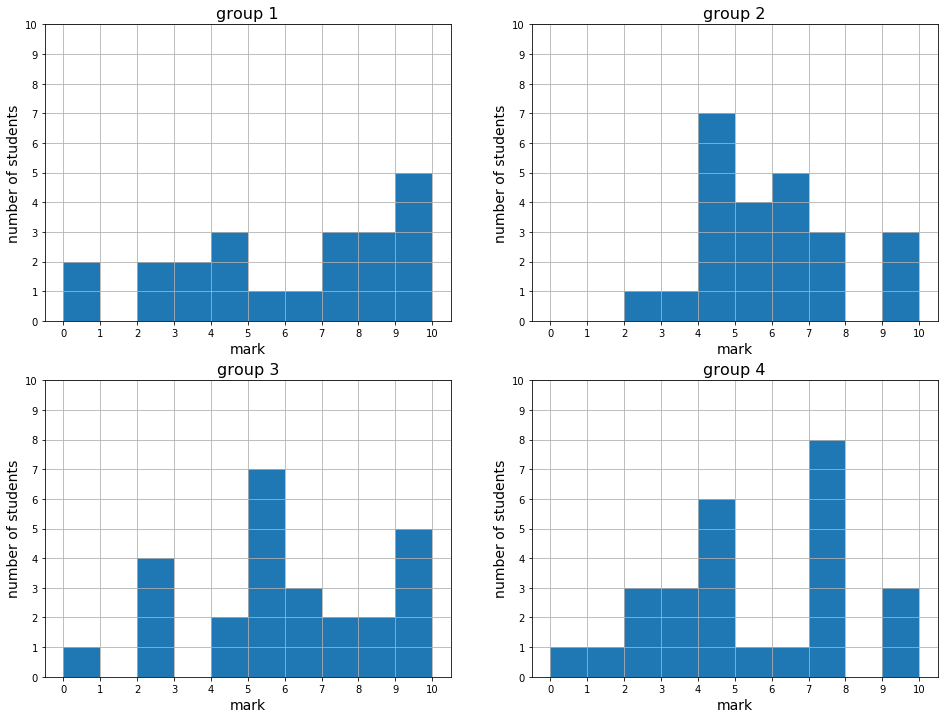
\includegraphics[width=\linewidth]{ex7_histograms.png}
\end{center}
\end{problem}

\begin{solution}
Проще всего по гистограмме с шагом $1$ определять, конечно же, моду: это то значение (их может быть несколько), которому соответствует самый высокий столбец. То есть мода для группы $1$ равна $mod_1 = 10$ (высота столбца $5$), $mod_2 = 5$ (высота столбца $7$), $mod_3 = 6$ (высота столбца $7$), $mod_4 = 8$ (высота столбца $8$).

Чтобы посчитать медиану, можно, например, выписать все оценки и найти среди них середину.
Для группы $1$ это будет выглядеть так:
$$
    1, 1, 3, 3, 4, 4, 5, 5, 5, 6, 7, 8, 8, 8, 9, 9, 9, 10, 10, 10, 10, 10
$$

Всего $22$ числа, в середине оказались $7$ и $8$, т.е. $med_1 = \frac{7 + 8}{2} = 7.5$.

Опять же, в случае с нашей гистограммой можно было не выписывать всё в явном виде, на самом деле, нам нужно только знать общее количество оценок в группе (чтобы вычислить, где находится середина) и понять, где эта середина расположена на графике.

Посчитаем медиану для группы $2$. Общее количество человек --- это суммарная высота всех столбцов на гистограмме, т.е. $1 + 1 + 7 + 4 + 5 + 3 + 3 = 24$. Значит, нам нужны столбцы с $12$-ой и $13$-ой по порядку оценкой (середина). Пройдёмся по гистограмме слева направо и посчитаем, сколько оценок встретилось: в столбце $2-3$ одна оценка, в столбцах $2-4$ две, в $2-5$ уже целых $9$. А в столбцах $2-6$ суммарно стало $13$ оценок. Значит, $12$-ая и $13$-ая оценка обе попадают в столбец $5-6$, т.е. $med_2 = \frac{6 + 6}{2} = 6$.

Аналогичным способом (любым из двух) можно посчитать медиану для оставшихся двух групп: $med_3 = \frac{6 + 6}{2} = 6$, $med_4 = 5$.

В итоге результаты такие:
\begin{align*}
    &mod_1 = 10 &med_1 = 7.5 \\
    &mod_2 = 5 &med_2 = 6 \\
    &mod_3 = 6 &med_3 = 6 \\
    &mod_4 = 8 &med_4 = 5
\end{align*}

Что можно сказать по полученным значениям и гистограммам? Например, что проверяющий группы $2$ неохотно ставит высокие оценки. А вот в группе $3$, казалось бы, довольно много студентов с оценкой $8$, но им это не помогло: только половина оценок превысила $5$.

Ради интереса можно посчитать среднее значение, которое не требуется в задании, потому что может занять чуть больше времени.
Например, посчитаем среднее для группы $1$. Для этого нам надо знать, сколько всего человек писали работу и сколько человек получило каждую оценку.

Посмотрим высоту каждого столбца, чтобы посчитать количество разных оценок: высота столбца $0-1$ равна $2$, т.е. оценку $1$ получило $2$ человека, по аналогии, оценку $2$ получило $0$ человек, $3$ --- $2$ человека, $4$ --- $2$ человека, $5$ --- $3$ человека и т.д.  Общее количество человек --- это суммарная высота всех столбцов на гистограмме, т.е. $2 + 0 + 2 + 2 + 3 + 1 + 1 + 3 + 3 + 5 = 22$.
Таким образом, средняя оценка в группе $1$ равна:
$$
\bar x_1 = \frac{1 \cdot 2 + 2 \cdot 0 + 3 \cdot 2 + 4 \cdot 2 + 5 \cdot 3 + 6 \cdot 1 + 7 \cdot 1 + 8 \cdot 3 + 9 \cdot 3 + 10 \cdot 5}{22} \approx 6.59
$$

Аналогично вычисляются средние оценки для остальных групп:
\begin{align*}
    mod_1 &= 10 &med_1 &= 7.5 &{\bar x_1} &\approx 6.6\\
    mod_2 &= 5 &med_2 &= 6 &{\bar x_2} &\approx 6.5\\
    mod_3 &= 6 &med_3 &= 6 &{\bar x_3} &\approx 6.5\\
    mod_4 &= 8 &med_4 &= 5 &{\bar x_4} &\approx 6.0
\end{align*}

Как видно, мода может оказаться левее среднего или медианы, а может -- правее. Точно так же, нельзя сказать, что медиана всегда будет больше или меньше среднего. Результат зависит от конкретного набора данных. Обычно считается, что хорошо, когда данные сконцентрированы вокруг среднего значения и не содержат выбросов, в этом случае все три статистики будут довольно близки.

\end{solution}

\todo[inline]{Упражнение на придумать дисперсию в модулях и медианах либо сказать устойчива ли она к выбросам - ???}

\todo[inline]{Задачка на то, кто обычно левее а кто правее (мода медиана среднее - ???}

\end{document}
